\documentclass[a4paper,12pt]{ctexart}

\usepackage{geometry}
\geometry{left=2.5cm,right=2.5cm,top=3cm,bottom=3cm}
\usepackage{graphicx}
\usepackage{booktabs}
\usepackage{longtable}
\usepackage{listings}
\usepackage{xcolor}
\usepackage{amsmath, amssymb}
\usepackage{hyperref}
\usepackage[normalem]{ulem}
\usepackage{listings}

\newcommand{\uText}[2][3cm]{\uline{\makebox[#1][c]{#2}}}

\hypersetup{
    colorlinks=true,
    linkcolor=blue,
    citecolor=blue,
    urlcolor=blue
}

\lstset{
    basicstyle=\ttfamily\small,
    numbers=left,
    numberstyle=\tiny,
    keywordstyle=\color{blue},
    commentstyle=\color{gray},
    stringstyle=\color{red},
    frame=single,
    breaklines=true,
    showstringspaces=false
}

\begin{document}

\begin{titlepage}
    \centering
    \vspace*{3cm}
    {\Huge\bf 系统开发工具基础实验报告\\[1.5cm]}
    {\Large\it 实验内容:\uText[4cm]{实验一}\\[0.5cm]}
    {\Large\it 姓名:\uText[4cm]{张家宜} \quad 学号:\uText[5cm]{2024020013045}\\[0.5cm]}
    {\Large\it 日期:\today\\[1.5cm]}
    \vfill
    \normalsize
    \vspace*{1cm}
\end{titlepage}

% 目录
\tableofcontents
\newpage

    
\section{练习内容}
\subsection{Latex文档编辑}
\subsubsection{\textbackslash documentclass}
\begin{lstlisting}[language=TeX]
\documentclass[a4paper, 12pt]{article}

\begin{document}
  A sentence of text.
\end{document}
\end{lstlisting}

\textbackslash documentclass 命令必须出现在每个 LaTeX 文档的开头。花括号内的文本指定了文档的类型。

\subsubsection{\textbackslash begin \& \textbackslash end}
\textbackslash begin\{document\} 和 \textbackslash end\{document\} 可以将文本内容包裹起来

\subsubsection{\textbackslash date}
\verb|\date{}可以在title里面显示时间|

使用\textbackslash today 可以显示当前的日期

\today

\subsubsection{\textbackslash title}
\begin{lstlisting}
\title{My First Document}
\author{My Name}
\date{\today}
\maketitle
\end{lstlisting}
\textbackslash maketitle 命令可以给文档创建标题。

\subsubsection{章节} \label{test}
\begin{lstlisting}
\section{Introduction}
This is the introduction.

\section{Methods}

\subsection{Stage 1}
The first part of the methods.

\subsection{Stage 2}
The second part of the methods.

\section{Results}
Here are my results.
\end{lstlisting}

\subsubsection{创建标签}
我在上一章里面添加了\textbackslash label\{test\},这里就可以使用\textbackslash red 和 \textbackslash pageref引用

Here are my results. Referring to section \ref{test} on page \pageref{test}

\subsubsection{生成目录}
\begin{lstlisting}
\pagenumbering{roman}
\tableofcontents
\newpage
\pagenumbering{arabic}
\end{lstlisting}

使用\textbackslash newpage会另起一页

\subsubsection{中文字体支持}
\verb|只需要在文档的前导命令部分添加:\usepackage[UTF8]{ctex}|

在overleaf里面还需要把文档的Compiler设置成XeLaTeX

\subsubsection{字体效果}
\begin{lstlisting}
\textit{words in italics} \textsl{words slanted} \textsc{words in smallcaps} \textbf{words
in bold} \texttt{words in teletype} \textsf{sans serif words} \textrm{roman
words} \underline{underlined words}
\end{lstlisting}

效果如下:

\textit{words in italics} \textsl{words slanted} \textsc{words in smallcaps} \textbf{words
in bold} \texttt{words in teletype} \textsf{sans serif words} \textrm{roman
words} \underline{underlined words}

\subsubsection{彩色字体}
\verb|{\color{colorname}text}|

其中 colorname 是颜色的名字,text 是彩色文本内容。

{\color{red}fire}

\textit{PS: 需要在 \textbackslash begin\{document\} 前输入 \textbackslash usepackage\{color\}}

\subsubsection{字体大小}
\begin{lstlisting}
normal size words {\tiny tiny words} {\scriptsize scriptsize words}
{\footnotesize footnotesize words} {\small small words} {\large large words}
{\Large Large words} {\LARGE LARGE words} {\huge huge words}
\end{lstlisting}

效果如下:

normal size words {\tiny tiny words} {\scriptsize scriptsize words}
{\footnotesize footnotesize words} {\small small words} {\large large words}
{\Large Large words} {\LARGE LARGE words} {\huge huge words}

\subsubsection{段落缩进}
\noindent 如果想要段落顶格,在要顶格的段落前加 \textbackslash noindent 命令即可。如果希望全局所有段落都顶格,在文档的某一位置使用 \textbackslash setlength\{\textbackslash parindent\}\{0pt\} 命令,之后的所有段落都会顶格。

\subsubsection{列表}
生成一个有序列表套无序列表
\begin{lstlisting}
\begin{enumerate}
  \item First thing
  \item Second thing
    \begin{itemize}
      \item A sub-thing
      \item Another sub-thing
      \item[+]加号
      \item[*]星号
    \end{itemize}
  \item Third thing
\end{enumerate}
\end{lstlisting}

\begin{enumerate}
  \item First thing
  \item Second thing
    \begin{itemize}
      \item A sub-thing
      \item Another sub-thing
      \item[+]加号
      \item[*]星号
    \end{itemize}
  \item Third thing
\end{enumerate}

\verb|\item[-] 会使用一个杠作为标志,你甚至可以使用一个单词,比如 \item[One]|

\subsubsection{注释和空格}
使用 \% 创建一个单行注释,在这个字符之后的该行上的内容都会被忽略,直到下一行开始。

%这是注释

多个连续空格在 LaTeX 中被视为一个空格。多个连续空行被视为一个空行。空行的主要功能是开始一个新的段落。通常来说,LaTeX 忽略空行和其他空白字符,两个反斜杠(\textbackslash \textbackslash)可以被用来换\\行。


\subsubsection{特殊字符}
\verb|在他们前面添加反斜杠进行转义 \# \$ \% \^{} \& \_ \{ \} \~{}|

\# \$ \% \^{} \& \_ \{ \} \~{}

\verb|反斜杠使用\textbackslash 命令代替。|

\subsubsection{表格}
\begin{tabular}{|l|l|}
  Apples       & Green  \\
  Strawberries & Red    \\
  Orange       & Orange \\
\end{tabular}

\vspace{14pt}

\begin{tabular}{rc}
  Apples              & Green  \\
  \hline                            %\hline 表示插入一个贯穿所有列的横着的分割线;
  Strawberries        & Red    \\
  \cline{1-1} Oranges & Orange \\   %\cline{1-1} 会在第一列和第二列插入一个横着的分割线
\end{tabular}

\vspace{14pt}

\begin{tabular}{|r|l|}
  \hline
  8              & here's \\
  \cline{2-2} 86 & stuff  \\
  \hline
  \hline
  2008           & now    \\
  \hline
\end{tabular}

\vspace{14pt}
尝试画出表格
\vspace{14pt}

\begin{tabular}{l|r|r}
    Item            &   Quantity    &   Price(\$)   \\
    \hline
    Nail            &   500         &   0.34        \\
    Wooden boards   &   100         &   4.00        \\
    Bricks          &   240         &   11.50       \\
\end{tabular}

\vspace{14pt}

\begin{tabular}{l|ccc}
    & Year \\
    \cline{2-4}
    City & 2006 & 2007 & 2008 \\
    \hline
    London & 21972 & 29713 & 29741 \\
    Berlin & 14102 & 28741 & 29104 \\
    Paris & 2919 & 291 & 2914
\end{tabular}{}

\newpage

\subsubsection{图表}
\begin{figure}[h!]
  \centering
  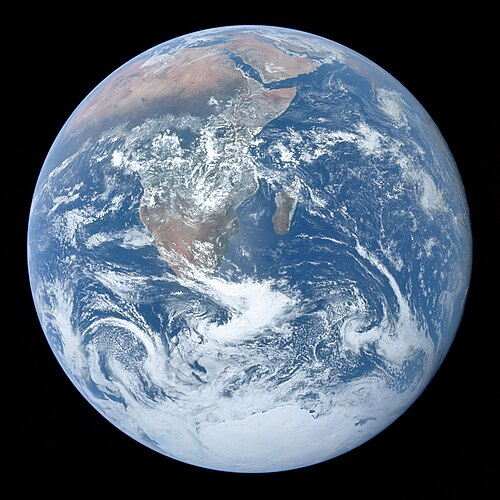
\includegraphics[width=1\textwidth]{marble.jpg}
  \caption{Here is my image}
  \label{image-myimage}
\end{figure}

\newpage

\subsubsection{公式}
$1+2=3$

\begin{equation}
    1+2=3
\end{equation}

\begin{eqnarray}
  a & = & b + c \\
  & = & y - z
\end{eqnarray}

$e^2$

$n_1$

$\frac{2}{3}$

$\sqrt{199}$

$$\sum_{x=1}^5 y^z$$

$$\int_a^b f(x)$$

$\delta, \Delta$

\subsection{版本控制(Git)}

\subsubsection{基础操作}
\begin{itemize}
  \item \texttt{git help <command>} \\ 查看某个 git 命令的帮助信息
  \item \texttt{git init} \\ 初始化一个新的仓库(生成 \texttt{.git} 目录)
  \item \texttt{git status} \\ 查看当前仓库状态(修改/暂存情况)
  \item \texttt{git add <file>} \\ 将文件加入暂存区
  \item \texttt{git commit} \\ 提交暂存区内容(注意撰写良好的提交信息)
\end{itemize}

\subsubsection{查看历史与差异}
\begin{itemize}
  \item \texttt{git log} \\ 查看提交历史
  \item \texttt{git log --all --graph --decorate} \\ 图形化显示提交与分支
  \item \texttt{git diff <file>} \\ 比较工作区与暂存区差异
  \item \texttt{git diff <rev> <file>} \\ 比较某文件在两个版本间的差异
  \item \texttt{git checkout <rev>} \\ 切换到某个提交或分支
\end{itemize}

\subsubsection{分支与合并}
\begin{itemize}
  \item \texttt{git branch} \\ 查看分支列表
  \item \texttt{git branch <name>} \\ 新建分支
  \item \texttt{git checkout -b <name>} \\ 新建并切换分支
  \item \texttt{git merge <rev>} \\ 合并指定提交/分支
  \item \texttt{git mergetool} \\ 使用工具解决冲突
  \item \texttt{git rebase} \\ 变基操作(重新应用提交)
\end{itemize}

\subsubsection{远端操作}
\begin{itemize}
  \item \texttt{git remote} \\ 查看远端仓库
  \item \texttt{git remote add <name> <url>} \\ 添加远端仓库
  \item \texttt{git push <remote> <local>:<remote>} \\ 推送本地分支到远端
  \item \texttt{git branch --set-upstream-to=<remote>/<branch>} \\ 建立本地与远端分支的关联
  \item \texttt{git fetch} \\ 获取远端更新(不合并)
  \item \texttt{git pull} \\ 获取并合并远端更新(= fetch + merge)
  \item \texttt{git clone <url>} \\ 克隆远端仓库
\end{itemize}

\subsubsection{撤销与修改}
\begin{itemize}
  \item \texttt{git commit --amend} \\ 修改最近一次提交
  \item \texttt{git reset}\\

\begin{table}[h]
\centering
\begin{tabular}{|c|c|}
\hline
\textbf{命令} & \textbf{效果} \\
\hline
\texttt{git reset --soft <commit>} & 撤销提交,但保留暂存区和工作区的改动 \\
\hline
\texttt{git reset --mixed <commit>} & 清空暂存区,保留工作区改动(默认模式) \\
\hline
\texttt{git reset --hard <commit>} & 提交、暂存区和工作区全部重置(不可恢复) \\
\hline
\end{tabular}
\caption{git reset 的三种模式对比}
\end{table}

  \item \texttt{git checkout -- <file>} \\ 丢弃工作区修改
\end{itemize}

\subsubsection{Git的课后练习}
\begin{enumerate}
    \item[2.1] git log --all --graph --decorate
    \item[2.2] git log -1 README.md
    \item[2.3] git blame \_config.yml | grep collections
    \item[3]\leavevmode\\
{
\begin{lstlisting}
git filter-branch --force \
  --index-filter 'git rm --cached --ignore-unmatch ./my_password' \
  --prune-empty \
  --tag-name-filter cat -- --all
\end{lstlisting}

filter-branch 用来改写仓库的历史

--index-filter 'git rm --cached --ignore-unmatch ./my\_password'

index-filter 会在历史的每一次提交里执行你指定的命令。

--prune-empty 有些提交可能唯一的改动就是那个密码文件。删掉后就变成“空提交”了,这个选项会自动删除这些空提交。

--tag-name-filter cat 保证 tag 还能继续指向正确的 commit

-- --all 表示要作用于所有分支和所有 tag
}
    \item[4] stash 就像一个临时抽屉,把改动存起来,工作区会恢复到干净状态

\end{enumerate}

\newpage

\section{解题感悟}

\LaTeX{} 是一款非常好用的排版工具。许多在传统编辑器中需要反复手动调整的格式与字体,在 \LaTeX{} 中常常只需改动几行代码即可完成;而且一旦抽象成模板,后续便能复用,事半功倍。对于在其他编辑器(如 Word)中较为麻烦的公式、表格等内容,只要掌握了基本方法,在 \LaTeX{} 里就能高效而规范地录入。

\vspace{14pt}

在项目开发中,Git 十分实用:它能有效进行版本控制,避免出现重大问题时无从挽回,同时也便利了调试与团队协作。正如 \cite{missing-semester} 所说:“尽管 Git 的接口有些丑陋,但是它的底层设计和思想却是非常优雅的。”

\newpage

\begin{thebibliography}{9}
\bibitem{missing-semester} Missing Semester 中文版,\url{https://missing-semester-cn.github.io/}
\bibitem{latex} OI-Wiki \LaTeX{} 工具,\url{https://oi-wiki.org/tools/latex/}
\end{thebibliography}

\section*{GitHub 链接}
\begin{center}
\href{https://github.com/Misasasasasaka/report}{https://github.com/Misasasasasaka/report}
\end{center}

\end{document}
